% !TEX root =  ../main_manuscript.tex 
\subsection{Statistical Methods}
The goal of the statistical analysis of the PRIAS data was to develop a model for predicting the time of disease reclassification in a personalized manner. To this end, for each patient we have the information about his age at the start of AS, all observed PSA measurements, and the time of the last negative biopsy. 

We start by specifying a model which extracts the underlying $\log_2\{\mbox{PSA + 1}\}$ profile of each patient from the observed PSA measurements. More specifically, we specify a linear mixed effects model with $\log_2\{\mbox{PSA + 1}\}$ as the outcome (see Outcome--2 in Figure \ref{fig:jm_blockdiag}). Our model uses a separate non-linear $\log_2\{\mbox{PSA + 1}\}$ profile over time, for each patient. It employs patient-specific random effects to account for correlation between $\log_2\{\mbox{PSA + 1}\}$ measurements of the same patient. However, the PSA measurements of a patient may be higher when measured closer to the time of reclassification. This is especially an issue because PSA measurements are missing (non-random) once a patient obtains disease reclassification. The vice versa, that is, disease reclassification may be predicted by looking at the PSA is also valid. To model this two-way effect, we specify a model for time of reclassification which shares the random effects used in the model for PSA (see Figure \ref{fig:jm_blockdiag}). Particularly, we use a relative risk model, wherein the hazard of reclassification utilizes the shared random effects indirectly, by depending on the fitted $\log_2\{\mbox{PSA + 1}\}$ value and velocity (rate of change). This connected specification of a linear mixed model and relative risk model is commonly known as a joint model for time-to-event and longitudinal data \citep{rizopoulos2012joint,tomer2019,coley2017prediction}.

\begin{figure}[!htb]
\centerline{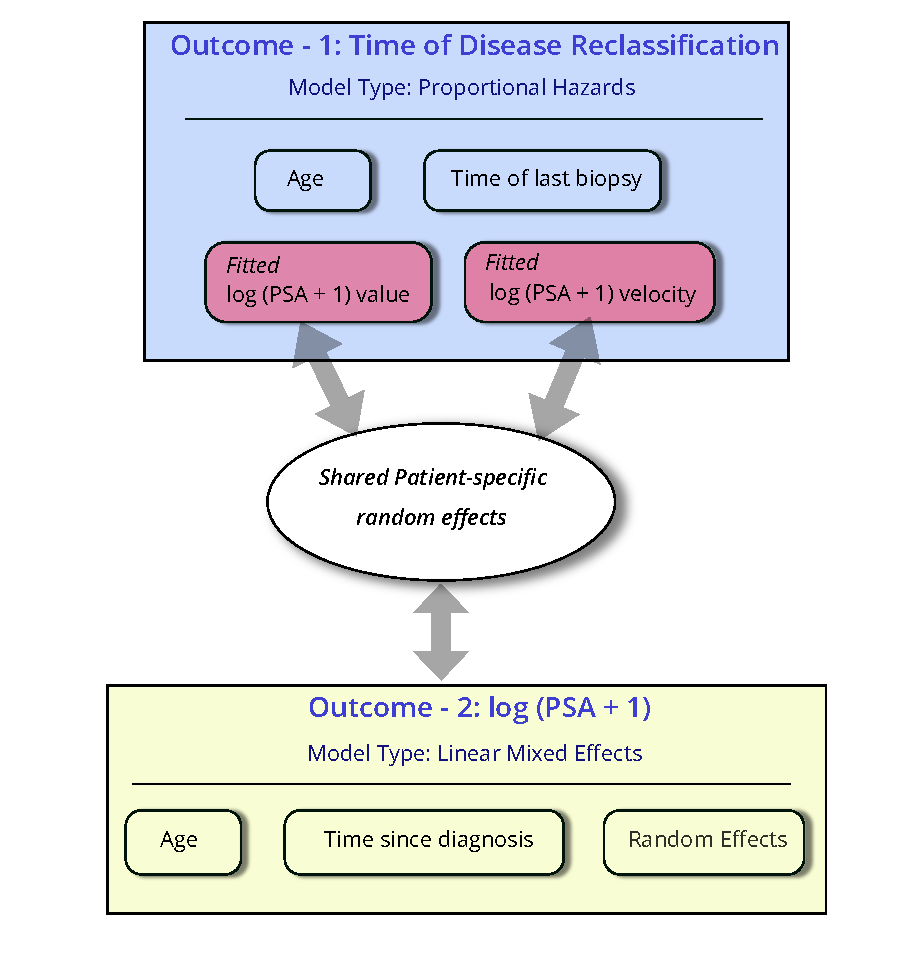
\includegraphics[width=\columnwidth]{images/jm_blockdiag.pdf}}
\caption{\textbf{Diagram of the joint model}: Per patient we observe the $\log_2\{\mbox{PSA + 1}\}$ transformed PSA, and the results of biopsies. We combine information from these observations to estimate the time of disease reclassification. To this end, we use a linear mixed effects model for $\log_2\{\mbox{PSA + 1}\}$ measurements, and proportional hazards model for time of disease reclassification. The time of disease reclassification depends on patient age, time of latest negative biopsy and underlying trend of PSA. To account for the correlation between PSA measurements and time of reclassification, the two models share patient-specific random effects in their model equations.}
\label{fig:jm_blockdiag}
\end{figure}

The consequence of such a joint model is that the shared random effects represent the unobservable state of PCa of each patient. On the other hand outcomes such as disease reclassification and PSA measurements are its observable manifestations. Such a shared random effect structure allows easy addition of more disease progression indicators (e.g., MRI information) when they are available in future. Furthermore, this structure also allows the follow-up schedule for outcomes/biopsies to depend on the observed values of each other. This is especially important because yearly biopsies in the PRIAS program are scheduled on the basis of the observed PSA doubling time of a patient.

We fit the joint model using the R package \textbf{JMbayes} \citep{rizopoulosJMbayes}. The package uses the Bayesian methodology to estimate model parameters. The model parameters and 95\% credible intervals are presented in Table.. of Appendix.

\subsection{Assessment of Predictions}
We assessed the goodness of fit of our model using both in-sample and out-of-sample predictions. For out-of-sample predictions we utilized the XX largest AS cohorts that constitute the GAP3 database \citep{gap3_2018}. That is, we used our model to predict disease reclassification in patients of other cohorts. The accuracy of these predictions were measured via the prediction error and the area under the receiver operating characteristic curves (AUC). The prediction error represents the difference between the true disease reclassification status of a patient, and the predicted risk of reclassification. Ideally this difference should be zero. On the other hand the AUC defines if the model is able to discriminate between patients who obtain reclassification versus those do not obtain reclassification. Ideally it should be equal to one. Since we work under a longitudinal study framework we compute these measures at a gap of every one year during the entire follow-up period.

\subsection{Decision Making Framework}
To assist patients and doctors in decision making for biopsies, we use the predicted risks of reclassification from our model. We calculate the probability if the patient will progress over the next ten years. We also provide an estimate of the number and time of biopsies that may be conducted, and the corresponding estimate of delay in detection of time of reclassification. Simultaneously, the patient is provided estimate of the number of time of biopsies with fixed schedule of biopsies. This allows patients to weigh harms and benefits of each strategy. We also implement this in a web-based risk calculator.